\documentclass[a4paper,12pt]{report}

% Différentes options pour la classe :
% - taille de la fonte    : 10pt, 11pt, 12pt
% - recto ou recto-verso    : oneside, twoside
% - stade de développement    : draft, final

% Chargement d'extensions
\usepackage[latin1,utf8]{inputenc}    % Pour utiliser les lettres accentuées
\usepackage[francais]{babel}    % Pour la langue française
\usepackage{graphicx}

% Informations le titre, le(s) auteur(s), la date
\title{Rapport de projet : Étrange}
\author {Caroline Keramsi, Florian Thorey, Samuel Mokrani}
\date{\today}

% Début du document
\begin{document}

\maketitle
\tableofcontents    % Table des matières
\listoffigures        % Liste des figures

\chapter{Introduction}

\section{Généralités}

{Dans le cadre du cours de System On Chips à Télécom Paristech, nous avons du réaliser
  un module de traitement vidéo. Plus précisément, ce module devait être capable à partir d'un flux vidéo d'entrée dont les intensités des pixels sont représentées en 256 niveaux de gris, donc codées sur 8 bits, d'établir une transformation géométrique d'ordre 3. Voici les images que nous pouvons obtenir suite à une telle transformation :}

  \begin{figure}[!h]
  \centering
  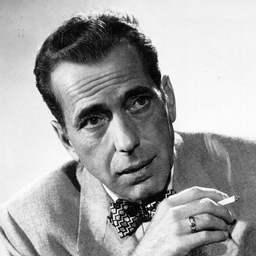
\includegraphics[scale = 0.5]{bogart.png}
  \caption{Image non transformée}
  \end{figure}

  \begin{figure}[!h]
  \centering
  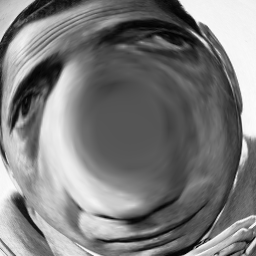
\includegraphics[scale = 0.5]{bogart_tr.png}
  \caption{Image transformée}
  \end{figure}

  \newpage

  \section{Le backward wrapping}

{Afin d'implémenter les transformations géométriques d'ordre 3 à appliquer au flux vidéo transitant par le module Étrange, la technique dite du "backward wrapping" est utilisée. Cette technique est très simple. Elle consiste à calculer pour chaque pixel de coordonnées $(X,Y)$ de l'image transformée les coordonnées $(x,y)$ de son antécédent dans l'image d'origine.
	 \newline
	 $$
	 x = a_{30}X^3 + a_{21}X^2Y + a_{12}XY^2 + a_{30}Y^3
	 + a_{20}X^2 + a_{11}XY  + a_{02}Y^2
	 + a_{10}X  + a_{01}Y
	 + a_{00}
  $$
	 $$
	 y = b_{30}X^3 + b_{21}X^23Y + b_{12}XY^2 + b_{30}Y^2
	 + b_{20}X^2 + b_{11}XY  + b_{02}Y^2
	 + b_{10}X  + b_{01}Y
	 + b_{00}
  $$

  {Dans ces formules, les $a_{ij}$ et $b_{ij}$ sont des coefficients réels. Ce qui implique que les coordonnées $(x,y)$ de l'antécédent dans l'image d'origine sont aussi des réels. Il peut donc s'agir d'un pixel fictif.
	 Il est donc nécessaire de procéder à une deuxième étape dîte d'interpolation afin de calculer l'intensité lumineuse que prendra le pixel de coordonnées $(X,Y)$ dans l'image transformée. Pour cela, on utilise les intensités lumineuses des quatre pixels les plus proches dans l'image d'origine pour en faire une interpolation bilinéaire. Ce qui nous donne la formule :
		\newline
		$$
		I = (1-dx).(1-dy).I_{00} + (1-dx).dy.I_{01} + dx.(1-dy).I_{10} + dx.dy.I_{11}
	 $$
		\newline
		Où les $dx$, $dy$ représentent respectivement les parties décimales de $x$ et $y$ et où les $I_{ij}$ représentent les intensités des 4 pixels voisins. Comme toute interpolation elle altère l'image mais nous jugeons que la qualité résultante est acceptable.
  }
  \section{Quelques précisions}
  {
	 Le flux à traiter est de 60 images par seconde au format $800*520$ pixels pour un format effectif de l'image de $640*480$ pixels en niveaux de gris codés sur 8bits. On en déduit que le débit entrant est de $800*520*60 = 25 Mo/s$
		\\
		\\
		Une contrainte supplémentaire est que la transformation de l'image doit s'effectuer tuile par tuile de taille $16*16$ pixels. Ainsi, il est possible de faire subir une transformation différente à chaque tuile présente dans l'image. L'image est donc composée de $40*30$ tuiles au format $16*16$ pixels, ce qui correspond à 1200 tuiles par image.
		\\
		\\
		Toutes les transformations opérées par le module Étrange doivent pouvoir être opérées en temps réel. Il s'agit d'une contrainte forte, le débit du flux vidéo entrant (25Mo/s) ne doit pas être altéré par les différentes opérations que subit l'image à travers Étrange.
		Ainsi, on dispose de 1/60ème de seconde pour traiter une image et donc $frac{1}{72000}^{eme}$ de seconde, soit $14 \mu s$ pour traiter une tuile.

		\section{Architecture retenue}
	 {Pour réaliser ce module de traitement vidéo, nous avons décidé d'utiliser l'architecture suivante :

		\begin{figure}[!h]
		  \centering
		  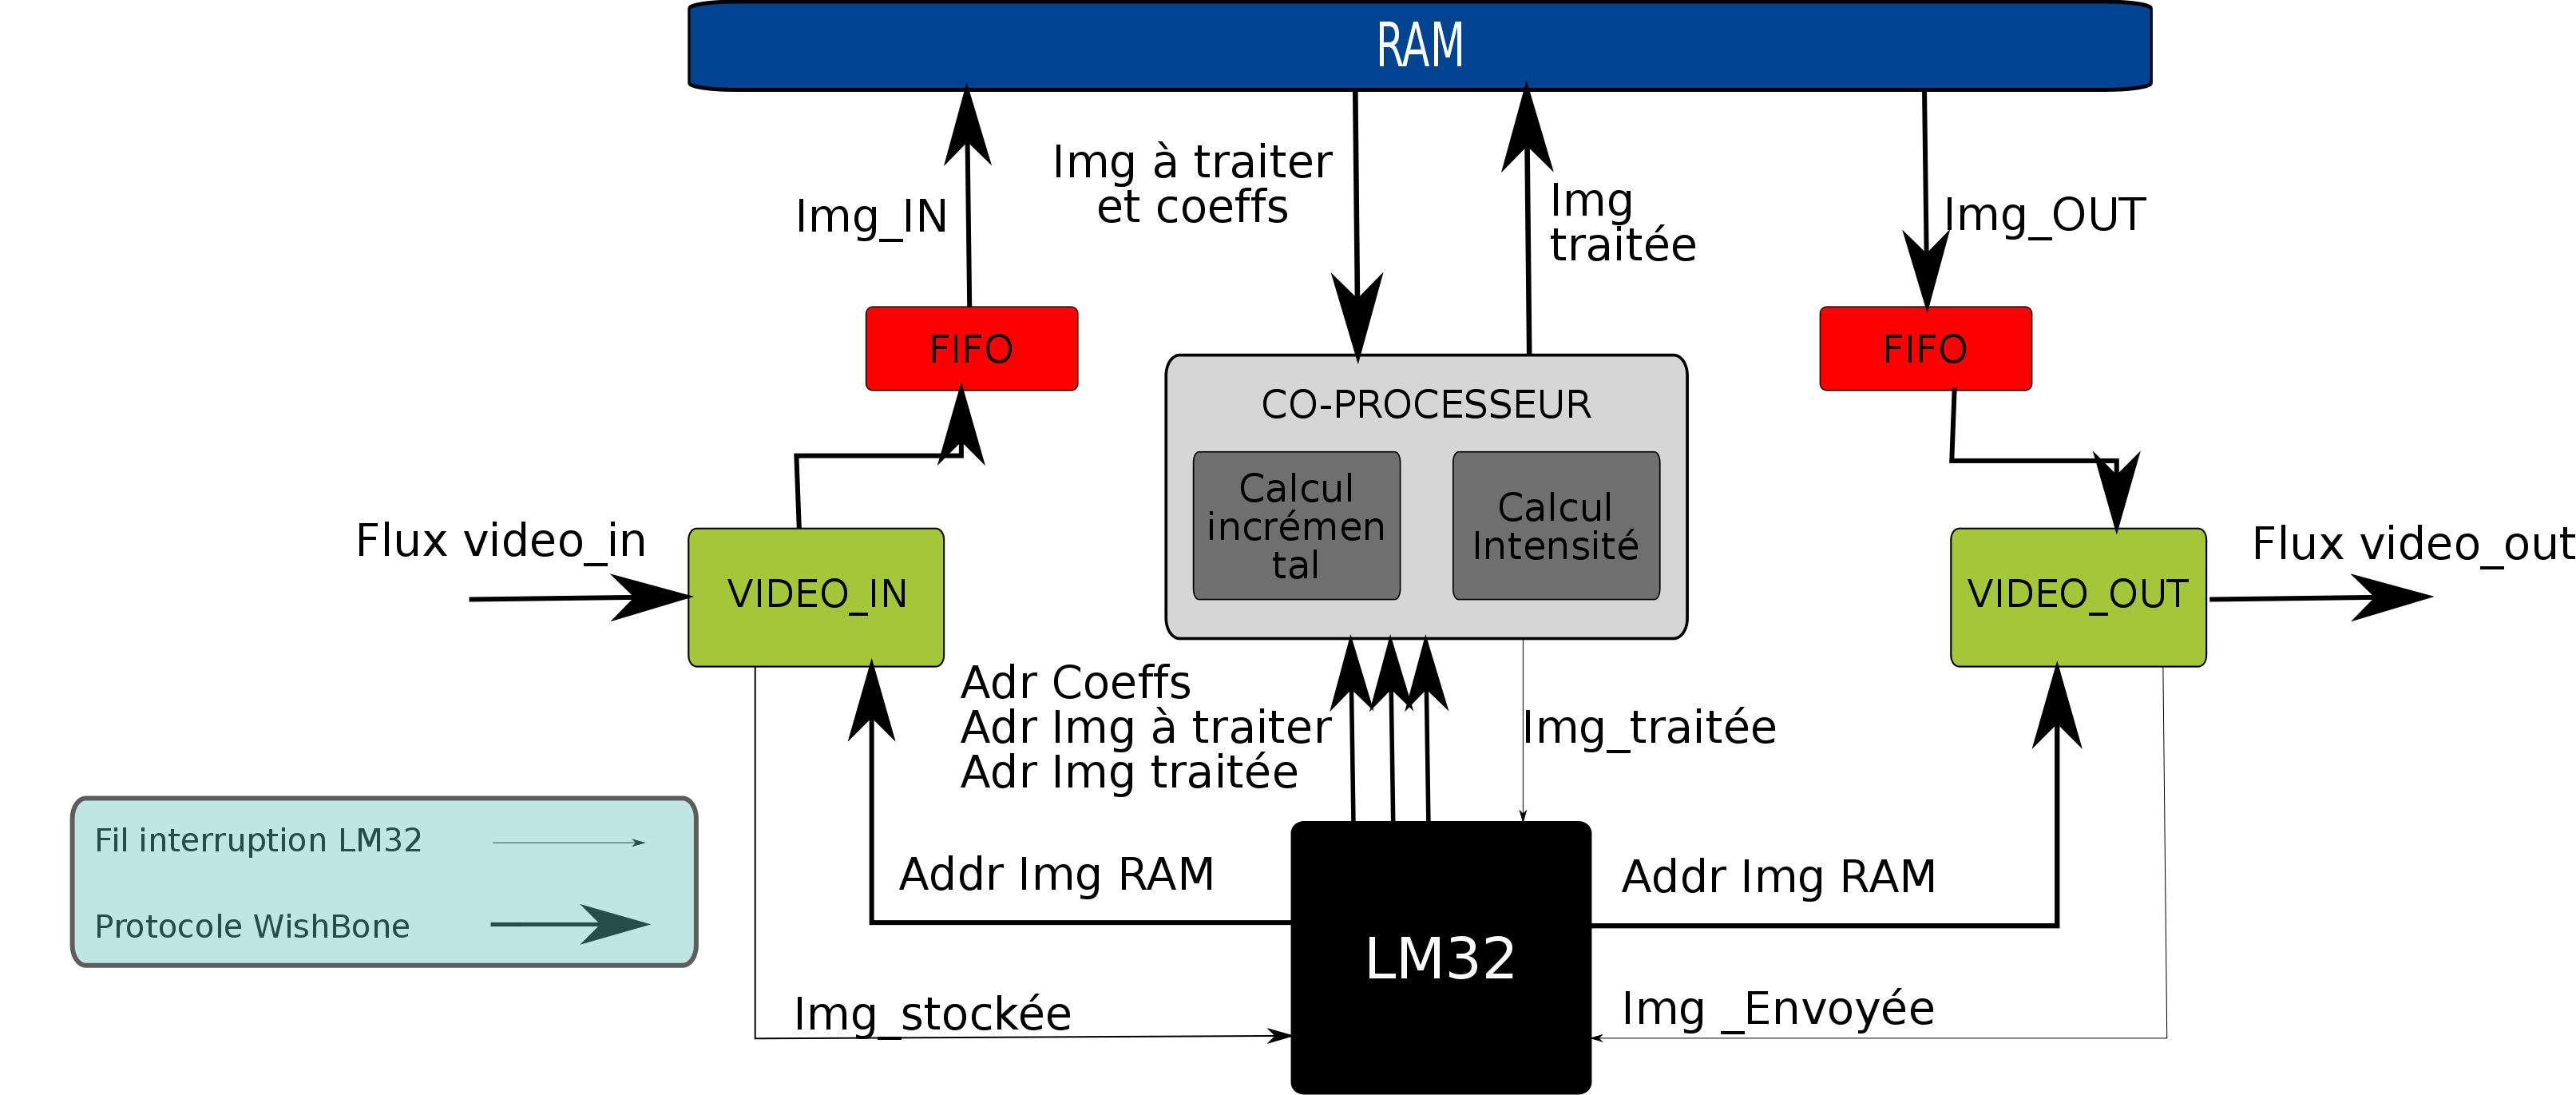
\includegraphics[scale = 0.1]{hardware-arch.png}
		\caption{Architecture}
		\end{figure}

		Le module Vidéo\_In se charge de mettre le flux entrant en RAM. Vidéo\_Calc se charge d'aller lire en RAM une image à traiter et à mettre à un autre endroit de la RAM l'image traitée. Enfin, le module Vidéo\_Out se charge d'aller lire l'image traitée et de générer un nouveau flux vidéo. Tous ces modules seront pilotés par le processeur (LM32) par le biais d'interruptions. Il enverra aux différents modules les bonnes adresses pour aller lire et écrire en RAM.\\ \\

		  Toutes les informations qui s'échangent entre les différentes composantes, le processeur, vidéo\_in, vidéo\_out et vidéo\_calc transitent via le bus Wishbone qui peut fonctionner à une cadence maximale de 100Mhz.\\ \\

		  Cette architecture a l'avantage d'être modulaire. Par exemple, on peut ne pas utiliser le module de transformation géométrique juste en changeant le programme tournant sur le processeur.
	 }



	 \chapter{Wb\_Slave / Vidéo\_In / Vidéo\_Out}
	 \section{Wb\_Slave}


	 \section{Vidéo\_In}

	 \begin{figure}[!h]
		\centering
		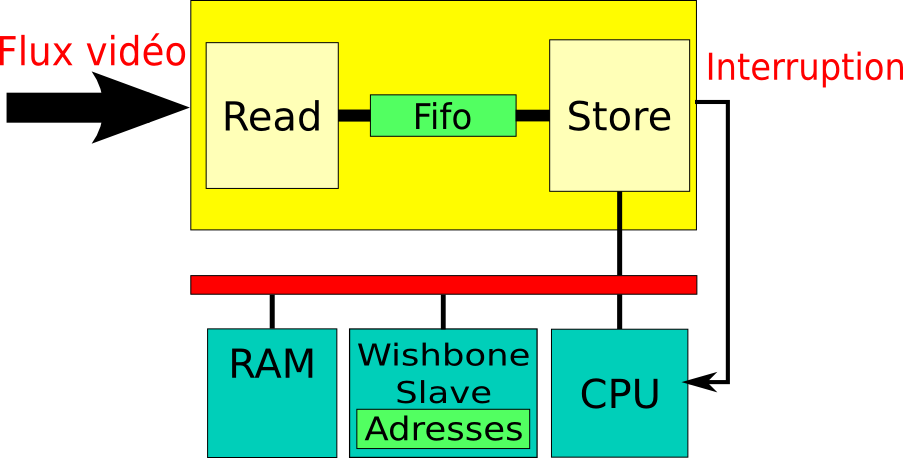
\includegraphics[scale = 0.5]{video_in.png}
	 \caption{Architecture de Vidéo\_In}
	 \end{figure}

	 Le rôle du module Vidéo\_In est de lire le flux vidéo entrant puis de stocker les images correspondantes en RAM à l'adresse spécifiée par le processeur.
		Vidéo\_In est constitué de deux sous-modules qui correspondent à ces deux fonctions et qui permettent de les exécuter en parallèle.


		\section*{Module read}
	 Ce module prend en entrée le flux vidéo constitué du pixel à lire sur 8 bits et des signaux de synchronisation \emph{line\_valid} et \emph{frame\_valid}.
		Lorsqu'il a détecté un pixel valide, il le place dans une fifo pour le mettre à disposition du module store.\\
		La synchronisation entre le module read et le module store est un point délicat.
		En effet la fifo contient uniquement des pixels et ne transportent aucune information concernant leur position dans l'image.

		\paragraph{SystemC}
	 En systemC, read est implémenté à l'aide d'un SC\_THREAD.
		Il peut ainsi disposer de ses propres compteurs qui lui permettent de se souvenir de la position
		du pixel courant dans le flux vidéo.
		Il peut ainsi détecter une incohérence sur le flux entrant (trop de pixels sur une ligne par exemple).\\
		La synchronisation avec store se fait à l'aide d'une variable de classe, \emph{first\_address}.
		Lorsque store a reçu sa première adresse, il passe ce booléen à vrai.
		Le thread read sait alors qu'il pourra commencer à stocker le flux entrant dans la fifo à partir du début de la prochaine image.\\
		La fifo est implémentée par une \emph{sc\_fifo}.
		L'écriture est donc un simple appel à la méthode d'écriture non bloquante \emph{nb\_write()}.
		Vidéo\_In ne peut pas attendre,
		si la fifo est pleine au moment de la tentative d'écriture, on sait que l'on ne tient pas le temps réel.

		  \paragraph{SystemVerilog}
	 La fonction read est implémentée en SystemVerilog par le module video\_in\_read qui est instancié dans le module video\_in.
		Son implémentation est très semblable au SystemC.\\
		On pourra noter une petite difficulté liée à l'utilisation de deux domaines d'horloge différents.
		La lecture des pixels entrant se fait sur l'horloge du flux vidéo à $25MHz$.
		La fifo, quant à elle fonctionne sur l'horloge système à $100MHz$.
		Une écriture dans la fifo se fait par le passage à 1 du signal \emph{w\_e}.
		Si on générait ce signal dans le bloc séquentiel chargé de la lecture et fonctionnant à $25MHz$,
			on risquerait d'écrire 4 fois dans la fifo au lieu d'une.
			  Pour régler cette difficulté, on génère dans ce bloc un signal \emph{write\_fifo\_slow}.
			  Un autre bloc séquentiel, fonctionnant sur l'horloge système, se charge de générer \emph{w\_e} lors de la
			  détection d'un front montant de \emph{write\_fifo\_slow}.


			  \section*{Module store}
	 Pour commencer, le module store attend que le processeur lui ait fourni une adresse. Pour ce faire il surveille le registre de contrôle du module wb\_slave
		qui lui est dédié. Quand celui-ci passe à 1, le module échantillonne le contenu du registre d'adresse réservé à Vidéo\_In. \\
		Store rentre ensuite dans la phase de stockage d'une image.
		Il attend que NB\_PACK pixels soient présents dans la fifo. Dès que c'est le cas, il les lit et les regroupe par paquets de 4, soit 32 bits,
			pour les stocker dans la RAM par une écriture wishbone bloc.
			  Lorsqu'il a fini d'écrire une image, le module envoie une interruption au CPU et se met en attente d'une nouvelle adresse.

			  \paragraph{SystemC}
	 Store est implémenté en SystemC par un SC\_THREAD.
		Ceci permet de se souvenir de l'état précédent du module.
		On peut donc décrire le comportement de store de façon séquentielle.
		Le fait de rester dans un état jusqu'à un certain événement est matérialisé par une boucle while contenant un ou plusieurs appels à wait(). \\
		La lecture dans la fifo est simple et se fait à l'aide de la méthode read() appliquée à la \emph{sc\_fifo}.

		\paragraph{SystemVerilog}
	 En SystemVerilog, il est nécessaire de changer complètement de paradigme.
		On ne peux pas attendre un événement à l'aide d'une boucle while,
			cela ne serait pas synthétisable!
			  Pour décrire un comportement similaire à celui réalisé en SystemC, on a donc mis en place une machine à états.




			  {}

	 \newpage

		\section{Vidéo\_Out}

	 \begin{figure}[!h]
		\centering
		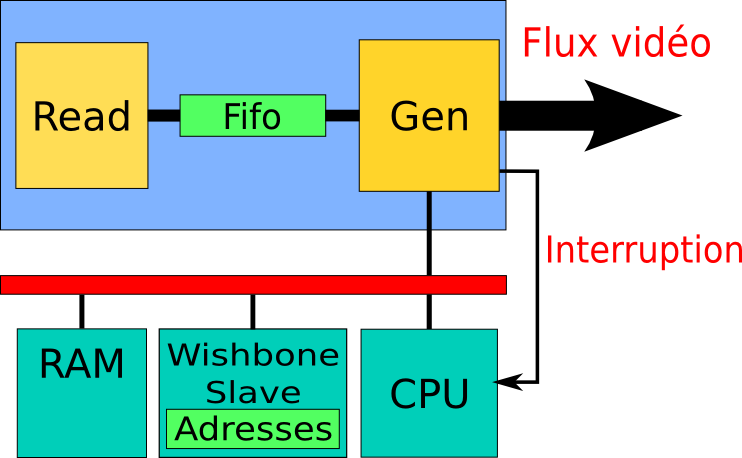
\includegraphics[scale = 0.5]{video_out.png}
	 \caption{Architecture de Vidéo\_Out}
	 \end{figure}

	 Le fonctionnement de Vidéo\_Out est exactement inverse à celui de Vidéo\_In.
		Il va chercher une image en RAM à une adresse indiquée par le processeur
		et génère le flux vidéo correspondant.
		Ces deux fonctions sont effectuées en parallèle par les deux sous-modules de Vidéo\_Out qui s'échangent
		les pixels au travers une fifo.

		\section*{Le module read}
	 Ce module va chercher les images en RAM et pose les pixels dans une fifo.
		Il attend que le processeur lui indique qu'une nouvelle adresse RAM est disponible en passant le registre de contrôle de wb\_slave, dédié à Vidéo\_Out, à 1.
		Il échantillonne alors le registre d'adresse de Vidéo\_Out.
		Une fois cette adresse obtenue, il va lire en RAM par paquets de NB\_PACK pixels, soit NB\_PACK/4 mots.
		À chaque paquet obtenu, les mots de 32 bits, découpés en pixel de 8 bits, sont placés dans la fifo dès qu'il y a de la place dans celle-ci.
		Une fois la lecture d'une image terminée, read se met en attente d'une nouvelle adresse.

		\paragraph{SystemC}
	 Le module est implémenté à l'aide d'un SC\_THREAD.
		Il effectue des écritures bloquantes sur la fifo.
		Sa vitesse est donc limitée par les lectures en RAM et
		par le rythme auquel le SC\_THREAD gen vide la fifo.

		\paragraph{SystemVerilog}
	 La problématique est la même que pour le module store de Vidéo\_In.
		Le style d'écriture en SystemC ne peut pas être reproduit en SystemVerilog.
		Le SC\_THREAD a donc été traduit sous la forme d'une machine à états dans le module video\_out\_read instancié par le module video\_out.

		\section*{le module gen}
	 Gen récupère les pixels qui ont été posés dans la fifo par le module read.
		Il génère ensuite le flux vidéo correspondant.

		\paragraph{SystemC}
	 Le code systemC est essentiellement une reprise de video\_gen.
		On réalise une lecture non bloquante de la fifo.
		Si la fifo est vide, on le détecte.
		On en déduit que l'on ne tient pas le temps réel.

		\paragraph{SystemVerilog}
	 Le module est implémenté à l'aide d'une machine à états.
		Celle-ci fonctionne avec l'horloge du flux vidéo, à 25 MHz.
		La lecture dans la fifo, qui fonctionne à 100 MHz doit donc se faire
		par l'intermédiaire d'un bloc séquentiel utilisant l'horloge système.
		Celui-ci génère le signal \emph{r\_ack} lorsqu'elle détecte le front montant
		du signal \emph{r\_ack\_slow} contrôlé à 25 MHz.


		\chapter{Vidéo\_Calc}

	 \section{Généralités}

	 Comme annoncé dans l'introduction, la transformation géométrique à appliquer au flux vidéo transitant par le module Étrange doit pouvoir être effectuée en temps réel, c'est à dire que tous les 1/60 de secondes, il faut qu'une nouvelle image puisse sortir du module. Le traitement par le processeur de la transformation d'ordre 3 par la technique du backward wrapping  à appliquer à l'image ne permet pas de tenir de tels timings. C'est pourquoi un coprocesseur est ajouté au module Étrange. Ce coprocesseur que nous avons désigné sous le terme vidéo\_calc est chargé d'implémenter cette technique présentée de manière détaillée dans l'introduction.
		\\
		\\
		Pour chaque tuile de taille $16*16$ pixels de l'image de sortie, on peut montrer que si l'on connait les coordonnées $(x,y)$ du pixel antécédent de celui de coordonnées $(X,Y)$ dans l'image de sortie, il est possible de déduire les coordonnées de l'antécédent de celui de coordonnées $(X+1,Y)$ en se basant uniquement sur les coordonnées de celui en $(X,Y)$. De plus, ce calcul peux s'effectuer à chaque cycle d'horloge.
		Ainsi, une fois connues les coordonnées $(x,y)$ de l'antécédent du pixel supérieur gauche d'une tuile de l'image de sortie, il est possible de calculer à chaque nouveau cycle d'horloge les coordonnées de tous les antécédents de la tuile. C'est la base du calcul incrémental.

		\section{Stockage}

	 \subsection*{Les coefficients}

	 Les coefficients pour chaque tuile de la transformation géométrique à appliquer au flux vidéo sont stockés en RAM à une adresse prédéfinie. Il y a donc 26 coefficients par tuile
		ce qui donne $26*1200 = 31200$ coefficients stockés en RAM. De plus pour chaque tuile, le processeur a placé en RAM les coordonnnées du rectangle circonscrit aux 4 antécédents des coins d'une tuile. Il y a donc en plus $2*1200 = 2400$ coordonnées.
		Les coefficients et les coordonnées sont stockés en RAM sur 32bits. Ce qui nous donne une place totale occupée de $(31200 + 2400)*4 = 134 Ko$

		\subsection*{Les images}

	 Les différents modules lisent et écrivent en RAM dans une zone occupant en tout 16 images (8 images non traitées et 8 images traitées). ce qui correspond à $16*640*480 = 5Mo$.

		\section{Fonctionnement}

	 Le module Vidéo\_Calc fonctionne selon le principe suivant :

		\begin{enumerate}

	 \item  Lorsqu'une nouvelle image est disponible en RAM. Le processeur envoie un signal, une adresse valide pour stocker l'image transformée afin d'initier le fonctionnement de Vidéo\_Calc ainsi d'une adresse pour lire une nouvelle image à traiter.

		\item Vidéo\_Calc va chercher en RAM les coefficients ainsi que les coordonnées de l'antécédent du coin supérieur gauche de la plus grande zone contenant les 4 antécédents des pixels des 4 coins de la tuile de l'image de sortie en cours de traitement.

		\item Vidéo\_Calc charge dans son cache une zone de $32*32 = 1024$ pixels ayant pour coin supérieur gauche les coordonnées récupérées au préalable. On considère que tous les antécédents se trouvent dans cette zone. Si malheureusement un des antécédents ne s'y trouve pas, alors il est perdu.

		\item En se basant sur le calcul incrémental déjà présenté, Vidéo\_Calc va calculer les antécédents de tous les pixels de la tuile en cours de traitement, si un pixel se trouve dans le cache alors on le récupère et  on effectue l'interpolation. Sinon on remplace ce pixel par un pixel blanc.

		\item Les pixels traités sont ensuite placés dans une fifo pour ensuite être stockés à nouveau en RAM à l'adresse spécifiée par le processeur lors de l'initialisation. L'utilisation d'une fifo permet de pipeliner d'une part les calculs et d'autre part le stockage en RAM.

		\end{enumerate}

	 \section{Architecture SystemC}
	 L'architecture en SystemC suit globalement le principe de fonctionnement. Ce module est constitué de 3 SC\_THREAD :

		\begin{enumerate}

	 \item get\_tile() : Ce processus est celui qui est chargé d'aller chercher les tuiles et de les charger dans le cache sur demande. ce processus s'occupe de plus de charger dans un buffer les coefficients propres à chaque tuile. Les accès de ce processus sur le bus Wishbone se font par paquets de 128 bits, soit 4 mots de 4 pixels.


	\item process\_tile() : C'est le processus de calcul de la transformation géométrique à proprement parlé : Pour chaque tuile de l'image de sortie, ce processus va demander à get\_tile() de charger le cache. Une fois le cache chargé, process\_tile() va effectué le calcul incrémental sur chaque pixel de la tuile de sortie, va regarder si ce pixel se trouve dans le cache, si oui il procède à l'interpolation puis place le pixel dans la fifo, sinon un pixel blanc est placé dans la fifo.


	\item store\_tile() : Comme son nom l'indique, la seule et unique tâche de ce processus est de récupérer les tuiles dans la fifo et de les stocker en RAM à la bonne place. Comme les  pixels font 8 bits et la taille du bus Wishbone ainsi que la taille des mots en mémoire  est de 32 bits, ce processus va faire des paquets de 4 pixels puis va aller écrire ces paquets en RAM 4 par 4.
\end{enumerate}

	 \section{Architecture SystemVerilog}
	 Nous n'avons pas eu le temps de terminer l'écriture du module Vidéo\_Calc en SystemVerilog, toutefois est présentée ici sous la forme d'un schéma l'architecture telle que nous l'avions imaginée. La problématique principale étant que le style d'écriture en SystemC n'est pas directement traduisible en SystemVerilog. Il est donc nécessaire de traduire sous la forme d'une machine à états les différentes intéractions se déroulant entre les 3 SC\_THREAD du SystemC.

		\begin{figure}[!h]
		\centering
		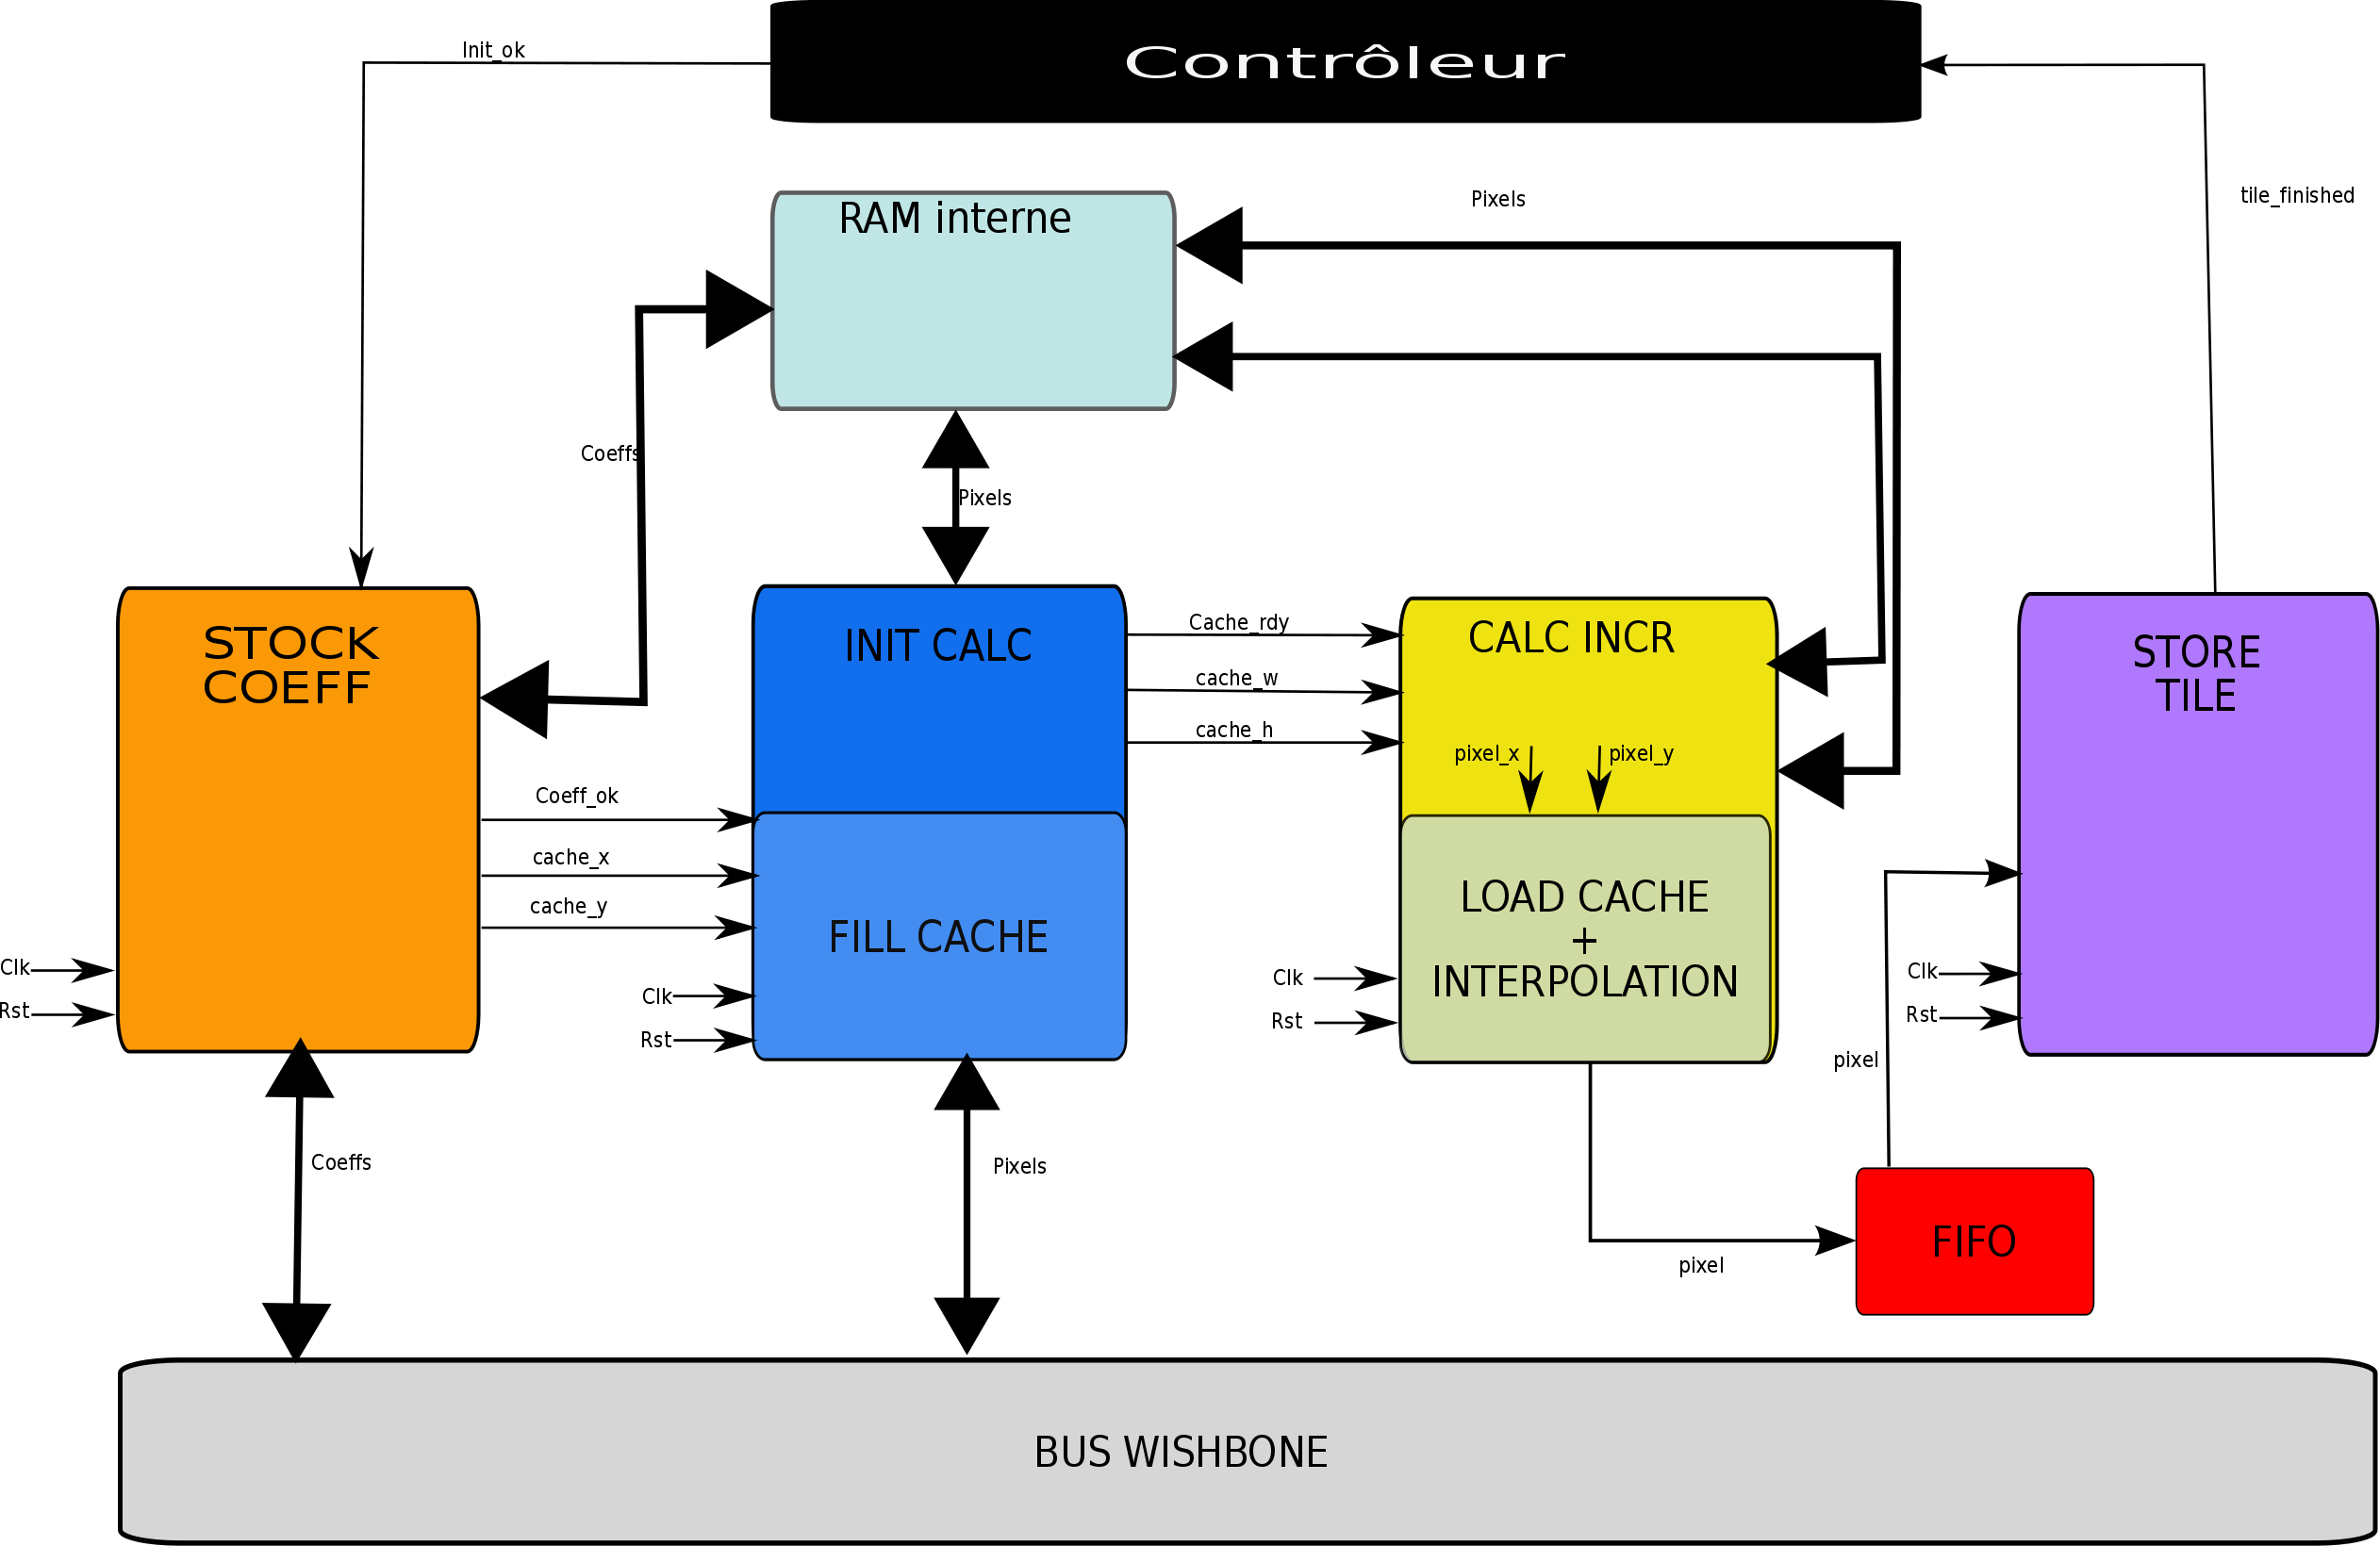
\includegraphics[scale = 0.15]{video_calc_verilog.png}
	 \caption{Architecture SystemVerilog Vidéo\_Calc}
	 \end{figure}

	 \chapter{Soft (LM32)}

	 \section{Les interruptions}

	 {Le processeur a la charge d'indiquer aux différents modules les adresses de lecture et d'écriture des différentes images. Plus précisément :

		\begin{itemize}
		\item à Video\_In : envoie de l'adresse où l'image entrante sera stockée
		  \item à Video\_Calc : \begin{itemize}
		\item envoie de l'adresse où sera lue l'image à traitée
		  \item envoie de l'adresse où sera stockée l'image traitée
		  \item envoie de l'adresse du début des coefficients pour le calcul incrémental
		  \end{itemize}
		\item à Video\_Out : envoie de l'adresse où sera lue l'image traitée
		  \end{itemize}

		Toutes ces adresses sont envoyées suites à des interruptions.
		  Il y a donc trois principaux handlers d'interruptions : Video\_In\_Handler, Video\_Out\_Handler et Video\_Calc\_Handler. \\ \\

		  Le processeur reçoit une interruption de Video\_In lorsque ce dernier a terminé de stocker une image en RAM. Le processeur lui envoit donc une nouvelle adresse pour stocker l'image suivante. Lors de cette interruption, il envoit aussi una adresse de lecture et de stockage à Video\_Calc.
		  Le processeur reçoit une interruption de Video\_Calc lorsque ce module a terminé de traiter une image. Si l'image traitée était la première, l'adresse de lecture de l'image traitée est envoyée à Video\_Out.
		  Le processeur reçoit une interruption de Video\_Out lorsque ce dernier a terminé de lire une image traitée en RAM. À ce moment là, il envoie une nouvelle adresse à Video\_Out.

		  Cet enchaînement fonctionne bien car le module Video\_Calc est plus rapide que Video\_In et Video\_Out.

	 }
	 \section{Gestion de la RAM}
	 {
		Pour stocker toutes ces images en RAM, on utilise un premier espace contenant les images stockées par Video\_In et un deuxième pour les images stockées par Video\_Calc. Nous pouvons illustrer l'état de la RAM par ce schéma :

		  \begin{figure}[!h]
		  \centering
		  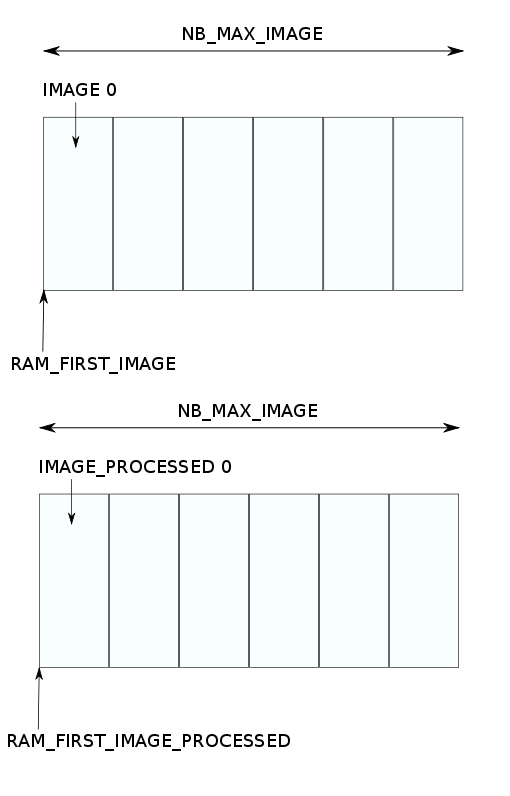
\includegraphics[scale = 0.3]{ram_management.png}
		\caption{État de la RAM}
		\end{figure}

	 }

	 \section{Initialisation des coefficients pour le calcul incrémental}
	 {La seconde fonctionnalité du processeur est de calculer tous les coefficients nécessaires au calcul incrémental effectué par le module Video\_Calc. Pour ceci, nous avons utilisé la représentation en virgule fixe pour que Video\_Calc puisse les récupérer en RAM et faire des calculs avec. Nous utilisons 16 bits pour représenter la partie entière et 16 bits pour la partie fractionnaire. Il y a plusieurs avantages à utiliser la représentation en virgule fixe. La première est que nous connaissons parfaitement la signification de chaque bits du nombre. La seconde est la rapidité des calculs comparée à l'utilisation de flottants.


		Pour que le module Video\_Calc puisse récupérer les coefficients en RAM calculés par le processeur, ce dernier lui envoit l'adresse de début de ces coefficients lorsqu'il envoit les adresses de lecture et d'écriture d'images dans Video\_Calc\_Handler.
	 }

	 \section{Calculs pour le chargement du cache}
	 {La dernière fonctionnalité du processeur est de calculer les quatre antécédents de chaque tuile et d'en déduire les coordonnées du pixel en haut à gauche du rectangle circonscrit à la partie de l'image qui représente l'antécédent de la tuile en question.
		Cette information est envoyée en même temps que les coefficients pour le calcul incrémental.

		  Ce calcul ne nous permet pas de gérer toutes les transformations possibles : ici, la première transformation se déroulera bien mais la deuxième échouera.
		  \begin{figure}[!h]
		  \centering
		  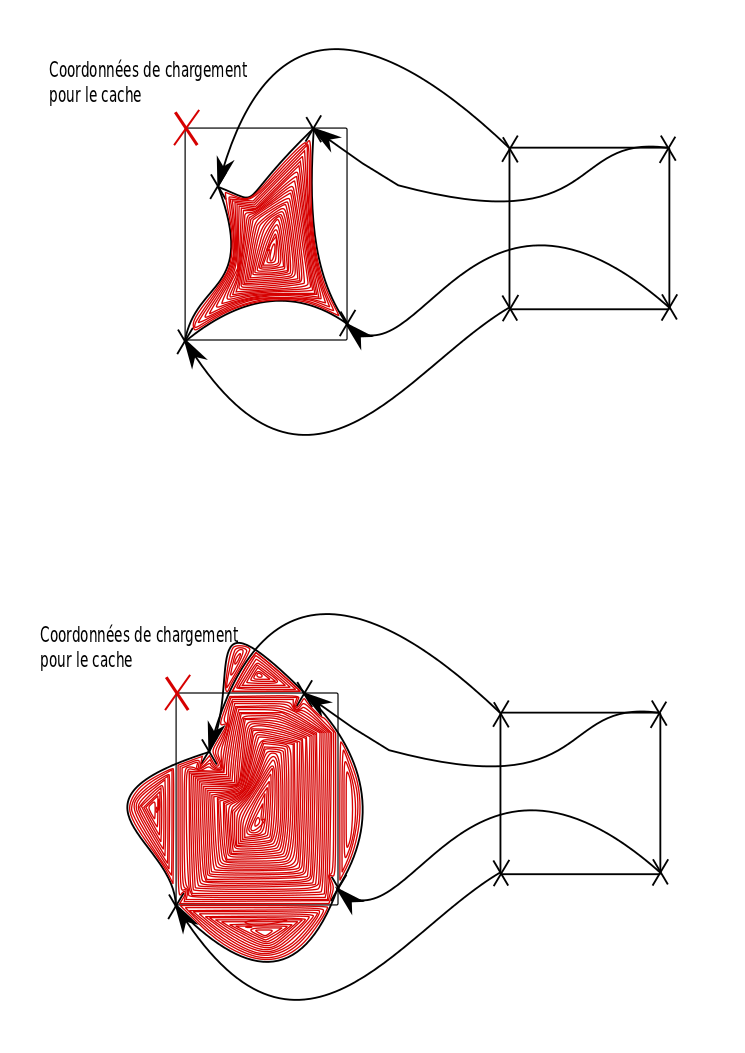
\includegraphics[scale = 0.3]{cache_proc.png}
		\caption{Chargement du cache}
		\end{figure}

	 }




	 \chapter{Conclusion}
	 { L'architecture décrite ci-dessus a été implémentée en SystemC dans un premier temps et nous arrivons à faire des transformations dans la limite de la gestion du cache.
On peut voir sur l'image ci-dessous un exemple de transformation contenant un zoom, une translation, une rotation et des termes d'ordre deux. Les pixels blancs représentent des antécédents n'étant pas en cache ou une intersection vide entre le cache et l'image car nous pouvons avoir des antécédents négatifs. Le résultat est plutôt satisfaisant même s'il y a des petits décalages de certaines tuiles par rapport aux autres.
		  \begin{figure}[!h]
		  \centering
		  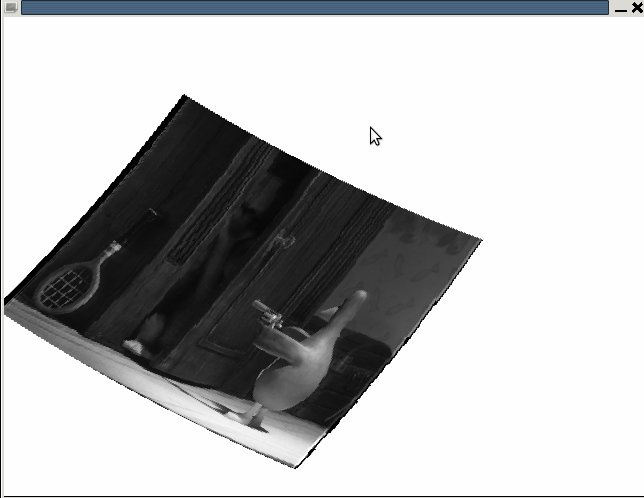
\includegraphics[scale = 0.3]{transfo.png}
		\caption{Exemple de transformation}
		\end{figure}

		La traduction en SystemVerilog n'est pas terminée. Vidéo\_In et Video\_Out sont fonctionnels en SystemVerilog mais Vidéo\_Calc n'a pas été traduit.\\ \\

		  Perspectives et améliorations :

		  \begin{itemize}
		\item Traduction de Video\_Calc en SystemVerilog
		  \item	Meilleure gestion du cache pour supporter des transformations plus complexes
		  \item Améliorer la partie interpolation car pour l'instant elle prend 4 cycles
		  \item Avoir des coefficients différents pour chaque tuile
		  \item La capacité de changer les coefficients pour le calcul incrémental par le clavier
		  \end{itemize}
	 }




	 % Fin du document
		\end{document}
